\documentclass[twocolumn]{article}
\usepackage[utf8]{inputenc}
\usepackage[pdftex]{graphicx} %per poter inserire le figure
\usepackage{SIunits}
\usepackage{tabularx}
\usepackage{indentfirst}
\usepackage{verbatim} % multiline commenting
\usepackage{subfig}
\usepackage{caption}
\usepackage{footmisc} % to \ref to footnotes
\usepackage{lipsum}
\usepackage{eucal}
\usepackage{eso-pic}
\usepackage{url}
\usepackage{bm}
\usepackage{afterpage}
\usepackage{parskip}
\usepackage{listings}
\usepackage{multicol}
\setlength{\columnsep}{1cm}
\usepackage{fancyhdr}
\usepackage{textcomp}
\usepackage{multicol}
\usepackage{multirow}
\usepackage{subfiles}
\usepackage{microtype}
\usepackage{adjustbox}
\usepackage{amsmath}
\usepackage{setspace}
\usepackage{wrapfig}
\usepackage{float}
\usepackage{array}
\usepackage{color}
\usepackage[toc,page]{appendix}
\usepackage{hyperref}
\usepackage{colortbl}
\usepackage{bbold}
\usepackage{booktabs} %linee tabelle
\usepackage[labelfont=bf,size=small]{caption} %didascalie
\usepackage[backend=biber]{biblatex}

\addbibresource{mybib.bib}   %file della bibliografia

\pagestyle{fancy} 

\newcommand{\gio}[1]{\textcolor{blue}{\textit{#1}}}

\definecolor{graytext}{HTML}{414141}
\definecolor{linkcolor}{rgb}{0,0,0.65} %hyperlink
\definecolor{linescolor}{rgb}{0.65,0.16,0.16}
\definecolor{cool}{RGB}{49,54,149}
\definecolor{hot}{RGB}{165,0,38}

\usepackage{fancyhdr} 

\pagestyle{fancyplain}
\fancyhf{}
\lhead{\ifnum\value{section}>0\nouppercase{\textbf{\leftmark}\fi}}
\rhead{De Bei, Lo Presti Piccolo, Piccolo}
\chead{}

\fancyfoot[R]{Page \thepage}
\fancyfoot[L]{\textit{Nanofabrication, Characterization and Modelling of Au Nanoparticles}}

\renewcommand{\headrulewidth}{0.2pt}
\renewcommand{\footrulewidth}{0.1pt}
\setlength\parindent{9pt} % To adjust the indentation

\title{}
\author{}
\date{}

\begin{document}

\thispagestyle{fancy}
\subfile{header.tex}
\thispagestyle{empty}

%\clearpage
\tableofcontents

\noindent\makebox[\linewidth]{\color{linescolor} \rule[-0.2cm]{0.85\paperwidth}{1pt}}
\noindent\makebox[\linewidth]{\color{linescolor} \rule[0.3cm]{0.85\paperwidth}{1.2 pt}}
%\pagebreak[4]

%\clearpage

\begin{multicols}{2}
\section{Introduction}
\noindent
Nanoparticle research has greatly expanded over the past decades. 
In particular, a major effort was put in the study and control of the shape and of the size of nanoparticles because of their influence over the electro-magnetic and optical properties of the nanoparticles.

Among noble metal nanoparticles, the Gold nanoparticles are of special interest due to their prominent optical resonance in the visible range.

The Au nanoparticles' interaction with light is strongly dictated by their environment, size and physical dimensions. Oscillating electric fields of a light ray propagating near a colloidal nanoparticle interact with the free electrons causing an oscillation of electron charge that is in resonance with the frequency of visible light. These resonant oscillations are known as surface plasmons. 

The aim of this work is to describe and characterize colloidal spherical gold nanoparticles. 

In the first part of this paper we will illustrate the main steps of the synthesis of the Au nanoparticles by means of the \textit{Turkevich method} (\textbf{Section \ref{sec:synthesis}}). 

After the synthesis we obtained the optical spectrum of the gold nanoparticles in the Vis-NIR range using a JASCO V670 spectrophotometer in order simulate the absorption line and the Mie extinction cross-section by means of the Mie theory in the dipolar approximation and of the size-corrected experimental dielectric function of Au (\textbf{Section \ref{sec:optic_char}}). 

The optical analysis of the gold nanoparticles allowed us to obtain informations on the size of the nanoparticles, on their concentration and on the refractive index of the medium.

We performed then independent measurements on the average size of spherical gold nanoparticles using the Grazing incidence X-Ray Diffraction (XRD): we estimated the diffraction of X-rays photons, coming from \(\text{Cu}_{k_\alpha}\), forming an angle of \(2\theta\) with respect to the incoming beam (\textbf{Section \ref{sec:XRD}}).

In the end, in \textbf{Section \ref{sec:SEM}}, we used a scanning electron microscope (SEM) to perform a statistical size distribution of the system.


\section{Synthesis of Au nanoparticles}
\label{sec:synthesis}
\noindent
Colloidal spherical gold nanoparticles can be synthesized via the Turkevich method: gold atoms are decomposed from a gold acid precursor forming a supersaturated solution and thus initiating the nucleation of the nanoparticles aggregating and growing under controlled constant temperature.

This method allowed us to synthetize nanoparticles of $10 \div 20 \,\nano\meter$ of diameters.

\subsection{Turkevich method}
The main steps which determine the Turkevich method can be summed up as follows:

\begin{enumerate}
    \item Pour in a beaker 9.5 mL of gold hydroclorate solution (HAuCl$_4$);
    \item Cover the beaker with the watch glass;
    \item Suspend the beaker in the crystallizer filled with normal water on the hot plate and rise the temperature up to 100\degreecelsius;
    \item Activate the stirrer in order to obtain an homogeneous distribution of temperature and concentration;
    \item Heat the sodium citrate solution (Na$_3$C$_6$H$_5$O$_7$) up to 100\degreecelsius;
    \item When both solutions are at 100 °C, add 0.5 mL of the Na$_3$C$_6$H$_5$O$_7$ solution to the beaker, which will decomposes the precursor by redox reduction in order to reduce gold atoms to metallic gold. The citrate concentration is chosen to prevent the formation of big structures;
    \item Wait 15 minutes with the stirrer on and at 100\degreecelsius.
\end{enumerate}

The result we obtained can be seen in \textbf{Figure \ref{fig:sample}}.

\begin{figure}[H]
    \centering
    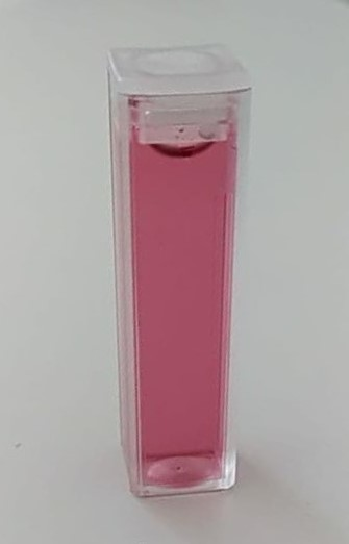
\includegraphics[width=0.45\linewidth]{image/data/turkevich.pdf}
    \caption{Sample of colloidal Au nanoparticles we obtained in the laboratory using the Turkevich method.}
    \label{fig:sample}
\end{figure}

\section{Optical Characterization}
\label{sec:optic_char}
\noindent
In order to acquire the optical spectrum of the colloidal Au nanoparticles we used a JASCO double beam spectrophotometer, which shines light in a continuous spectrum in the Vis-NIR range ($300\div 2700\, \nano\meter $).

To verify the presence of the localized surface plasmon resonance (LSPR) we acquired the absorbance spectrum: the spectrophotometer shoots on the sample a single wavelength at a time which is selected by a monocromator and then the same procedure is repeated for a second beam, which provides a base-
line. At this point the trasmittance $T$ is measured and then converted, using the Lambert-Beer equation (Equation \ref{eq:absorbance}), into absorbance data ($A$): 

\begin{equation}
    A:=\log_{10}\frac{1}{T}=\log_{10}(e)z \sigma_{ext} \rho
    \label{eq:absorbance}
\end{equation}

\noindent
where $z=1\, cm$ is the length of the sample, $\sigma_{ext}$ is the Mie extinction cross section and $\rho$ is the density of the nanoparticles.

The experimental data we obtained are plotted in \textbf{Figure \ref{fig:exp_data}}. As can be seen, the spectrum exhibits a resonant behavior, and data near the peak can be used to estimate various properties of the system.

\begin{figure}[H]
    \centering
    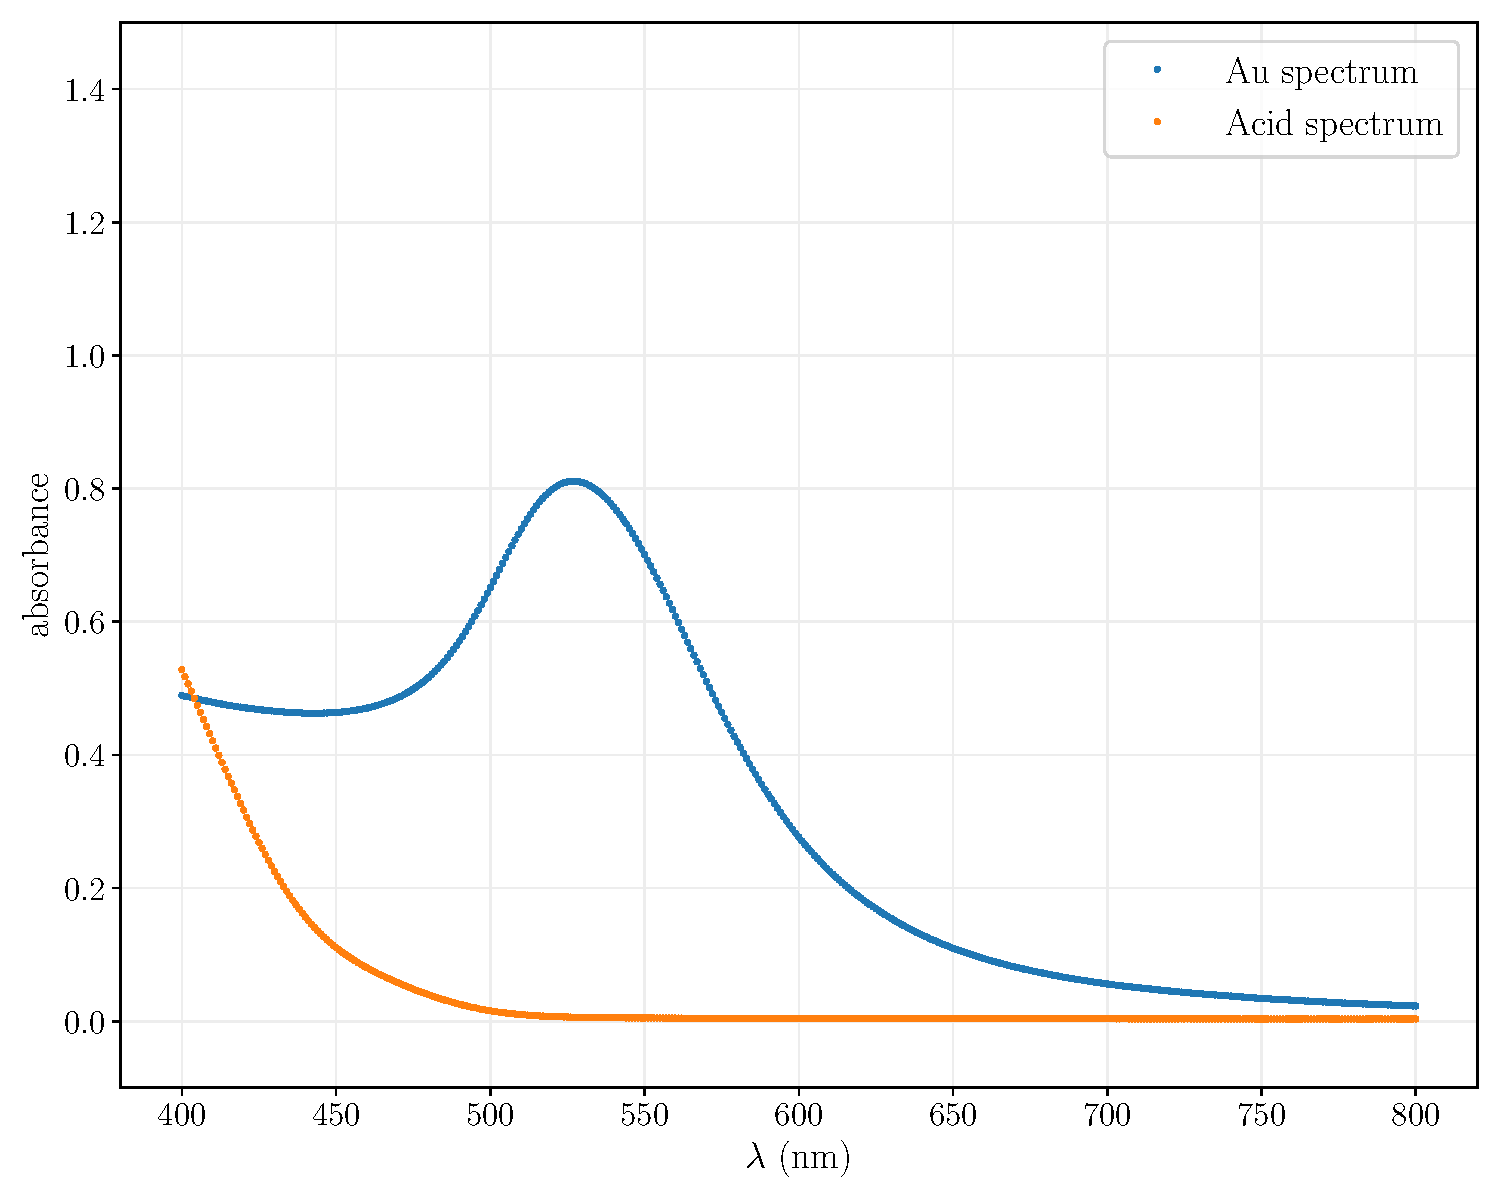
\includegraphics[width=\linewidth]{image/data/exp_data.pdf}
    \caption{Experimental spectra: in blue is plotted the Gold nanoparticle experimental spectrum, while in orange the acid spectrum.}
    \label{fig:exp_data}
\end{figure}

The label \textit{Acid spectrum} of \textbf{Figure \ref{fig:exp_data}} refers to the fact that in the first place we measured the optical spectrum of the medium in which nanoparticles were immersed, (which was water and tetrachloroauric acid),  and then we acquired the gold
nanoparticle solution spectrum (\textit{Au spectrum} label).

The following optical analysis has been performed in the $400 \div 800\,\nano\meter$ range.

\subsection{Model}
In order to apply the Mie theory in the dipolar approximation to the collected experimental data and in order to compute the extinction cross section we assumed some hypothesis on our physical system: first of all we supposed that the radius of the Au nanoparticles was much smaller with respect to the incident wavelengths ($R\ll \lambda$) and that the medium dielectric function was real ($\epsilon_m(\omega) \in \mathbb{R}$: non-absorbing matrix hypothesis). 

Furthermore, we supposed that the nanoparticles had spherical shape, that the system was monodispersed with respect to the particle radius and that the gold nanoparticles had a non real and size-dependent dielectric function $\epsilon(\omega) = \epsilon_1(\omega) +i\epsilon_2(\omega)$\footnote{In first approximation we can assume that dielectric function to be equal to the one computed by Johnson and Christy, see \textbf{Figure \ref{fig:size_correction}}. In addition, $\omega=c/\lambda$ and $c$ is the speed of light.}, described by the following equation:

    \begin{small}
    \begin{equation*}
    \begin{split}
       \epsilon(\omega,R) & = \epsilon(\omega,\infty) + \omega_P^2 \left(\frac{1}{\omega^2+\Gamma_{bulk}^2}-\frac{1}{\omega^2+ \Gamma(R)^2}\right) \\ 
     & -i\frac{\omega_P^2}{\omega} \left(\frac{\Gamma_{bulk}}{\omega^2+\Gamma_{bulk}^2}-\frac{\Gamma(R)}{\omega^2+ \Gamma(R)^2}\right)
      \end{split}
      \label{eq:epsilon}
    \end{equation*}
    \end{small}

\noindent
where $\epsilon(\omega, \infty)$ is the bulk dielectric function, $\omega_P$ is the plasmon frequency of bulk gold and $\Gamma$ is the typical damping time for the electrons.\\

\noindent
In particular, according to the Drude model, 

\[\Gamma(R)=\Gamma_{bulk}+q \frac{v_{F}}{R}\]

\noindent
where $q=\pi/4$ in the assumption of spherical nanoparticles, $v_F$ is the Fermi velocity for gold electrons, $R$ is the nanoparticle's radius, $\Gamma(R)$ is the size-dependent electrons relaxation frequency and $\Gamma_{bulk}$ is the relaxation frequency in bulk gold. 

In \textbf{Table \ref{tab:bulk_const}} we report the bulk constants of gold used in this work. 

\begin{table}[H]
    \centering
    \caption{Bulk constants of gold at room temperature.}
    \begin{tabular}{ccc}
    \toprule
      \bm{$\omega_p$}  \cite{Kittel2004}  & \bm{$\Gamma_{bulk}$}  \cite{Kittel2004} & \bm{$v_{F}$} \cite{Ashcroft76} \\
    \midrule
      $1.38 \cdot 10^{16} \,\text{Hz} $   & $1.08 \cdot 10^{14} \,\text{Hz}$ & $1.40 \cdot 10^6 \, \meter/\text{s}$ \\
    \bottomrule
    \end{tabular}
    \label{tab:bulk_const}
\end{table}

\noindent
In order to obtain the size-dependent dielectric function equation we have to apply a semi-classical correction: from the Drude model for the electrons we can derive that
$$
\begin{array}{l}
\epsilon_{1}(\omega, R)=\epsilon_{1}(\infty)+\omega_{p}^{2}\left(\frac{1}{\omega^{2}+\Gamma_{bulk}^{2}}-\frac{1}{\omega^{2}+\Gamma(R)^{2}}\right) \\
\epsilon_{2}(\omega, R)=\epsilon_{2}(\infty)-\frac{\omega_{p}^{2}}{\omega}\left(\frac{\Gamma_{bulk}}{\omega^{2}+\Gamma_{bulk}^{2}}-\frac{\Gamma(R)}{\omega^{2}+\Gamma(R)^{2}}\right)
\end{array}
$$

\noindent
We can observe the effects of the size correction of the dielectric function in \textbf{Figure \ref{fig:size_correction}} for different values of the radius. With the plot label \textit{Johnson and Christy} we refer to non size corrected values of the dielectric function.

From the second part of Equation \ref{eq:absorbance} we can express the absorbance $A$ as a function of the Mie extinction cross section as follows.

\noindent
Given that (quasi-static field approximation):
\begin{equation}
\sigma_{e x t}=9 \frac{\omega}{c} \varepsilon_{m}{ }^{3 / 2} \mathrm{~V} \frac{\varepsilon_{2}}{\left(\varepsilon_{1}+2 \varepsilon_{m}\right)^{2}+\left(\varepsilon_{2}\right)^{2}}
\end{equation}

\noindent
where $V$ is the nanoparticles' volume, we can use \textbf{Equation \ref{eq:absorbance}} and the spherical nanoparticles approximation to write $A$ as:

\begin{equation}
    A=K\epsilon_m^{3/2}R^3\rho\frac{\epsilon_2}{(\epsilon_1 + 2\epsilon_m)^2 + (\epsilon_2)^2}
    \label{eq:ass}
\end{equation}
with $K=\log_{10}(e)\frac{9}{c}\frac{4\pi}{3}z$.

\end{multicols}

\begin{figure}[H]
    \begin{minipage}[l]{1.0\columnwidth}
    \centering
    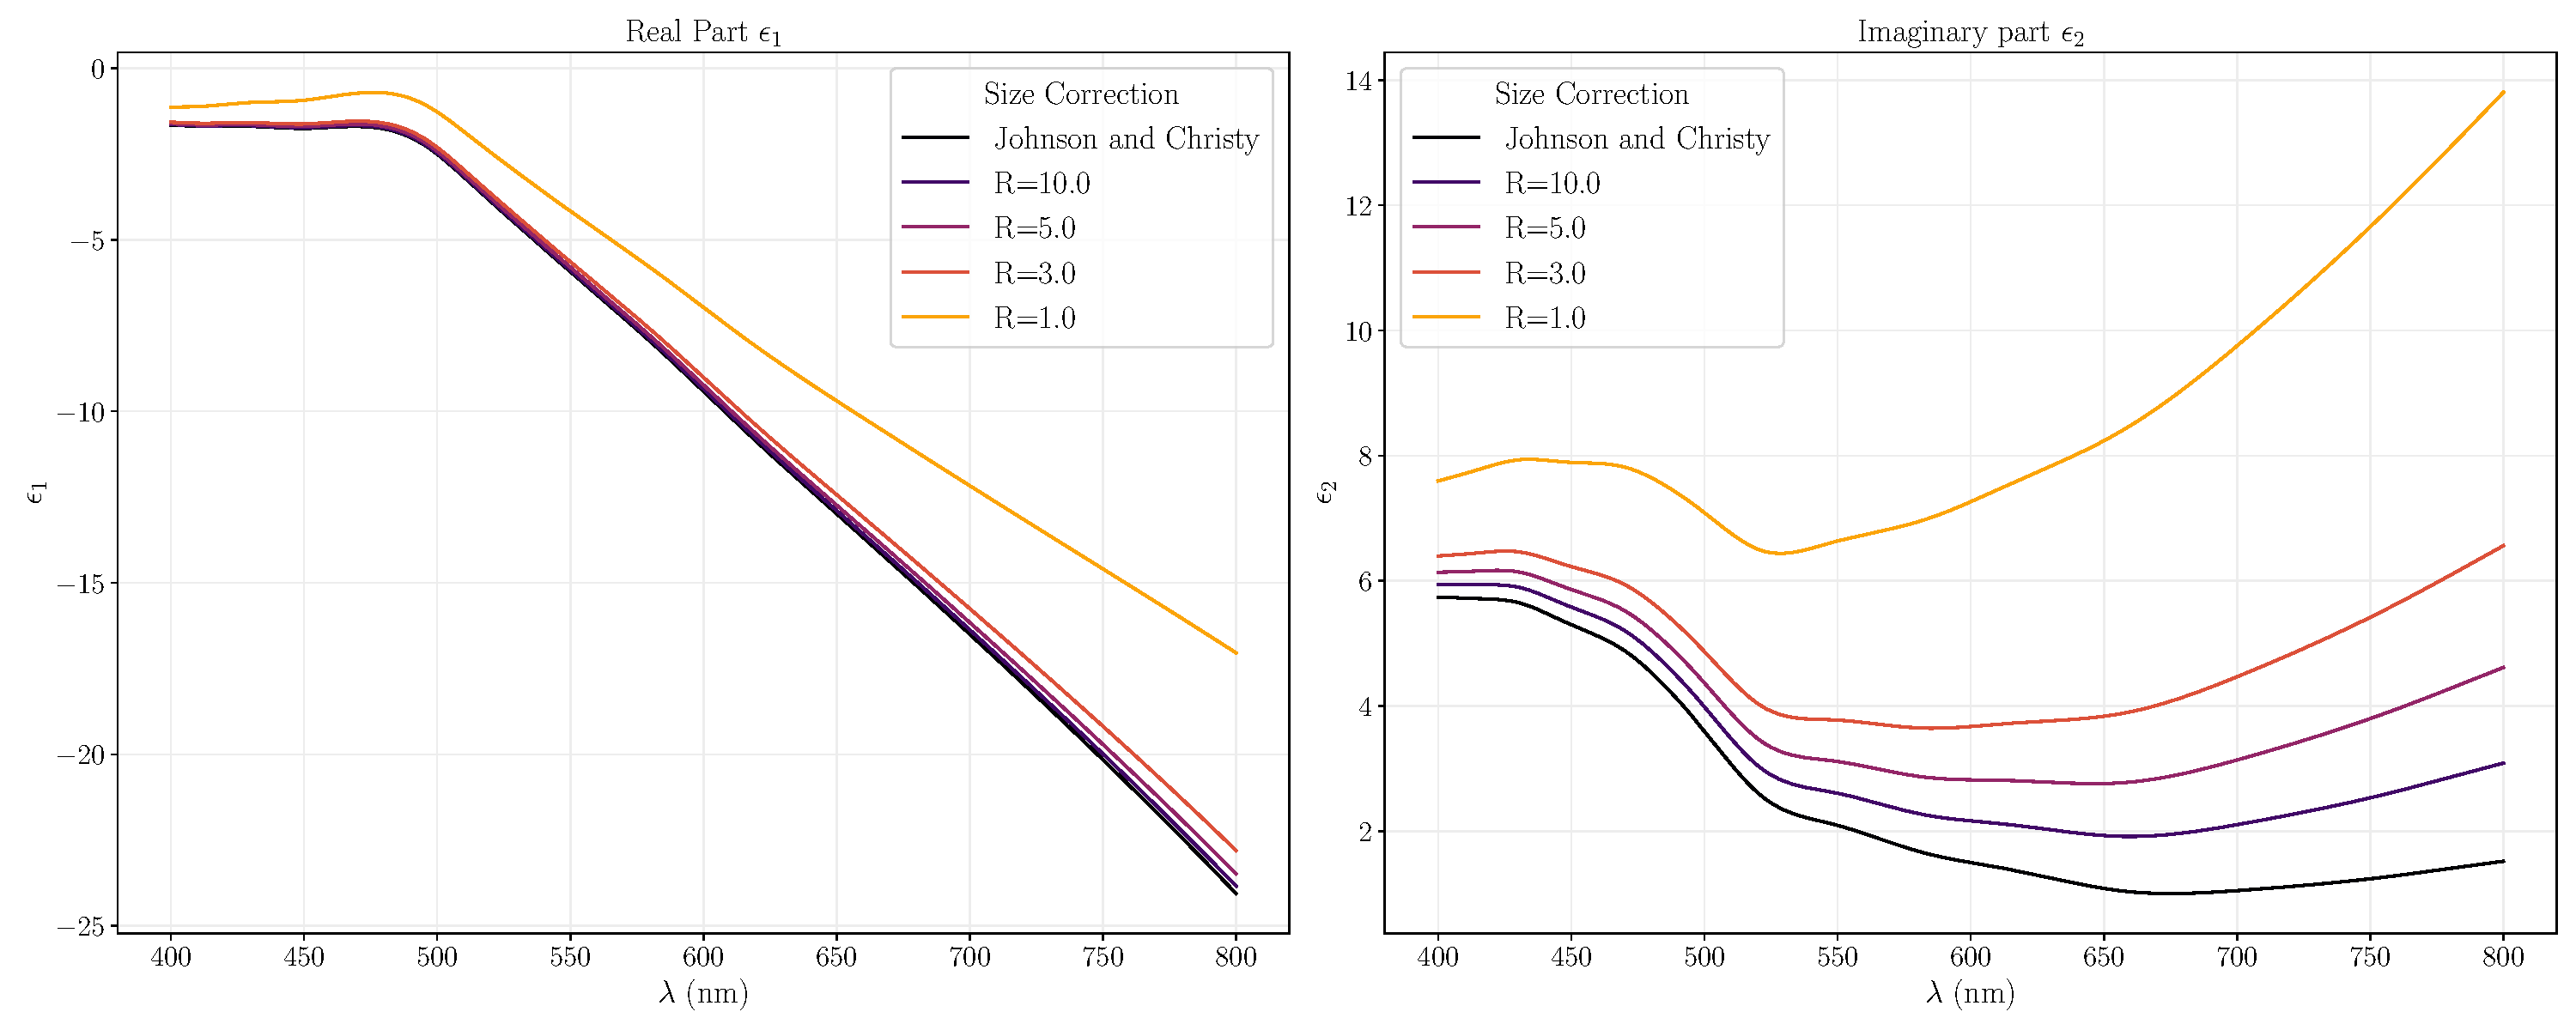
\includegraphics[width=\textwidth]{image/data/size_correction.pdf}
    \caption{Size correction of the dielectric function for different values of the radius. Johnson and Christhy label refers to non size corrected dielectric values.}
    \label{fig:size_correction}
    \end{minipage}
\end{figure}

\begin{multicols}{2}

Due to the fact of the presence of the $R^3\rho$ term in \textbf{Equation \ref{eq:ass}}, we have performed the optical analysis of the colloidal Au nanoparticles using from the beginning the size-dependent equation for the dielectric function i.e. using $\epsilon_1(\omega)$ and $\epsilon_2(\omega)$.

At this point we can model our system by varying its three free parameters ($\epsilon_m, \rho, R$).

In order to find the best-fit parameters, we began our analysis by varying $R$ and by keeping $\rho$ and $\epsilon_m$ constant obtaining the fit for the couple ($R,\rho$). At this point we estimated the stability basin of the best fit result by computing the minimized $\chi^2$, i.e.:

 \begin{equation}
        \chi^2 = (\frac{A_{exp}-A_{sim}}{\sigma_{A_{exp}}})^2, \quad \sigma_{A_{exp}} =\frac{1}{A_{exp}} 
\end{equation}

where $\sigma_{A_{exp}}$ is the error associated to the experimental absorbance\footnote{We choose this value for the error in order to give a different weight to the spectrum values and eventually obtain a better agreement between data and simulation.}. 


To obtain information on the stability of the best-fit parameters,
calculate and plot the $\chi^{2}$ values for different couples $(R, \varrho)$ and $\left(R, \varepsilon_{m}\right)$
and estimate the stability basin of your best fit result

Where $\epsilon_m = 1.33^2$ which is the refractive inde of water to the square


\newpage

\begin{itemize}
    \item at first, we vary R and $\rho$ keeping $\epsilon_m$ constant. Thus, we obtain the fit for the couple $(R,\rho)$; 
    \item then, we find the values minimizing the $\chi^2$ function, which is defined as follow:
        \begin{equation}
        \chi^2 = (\frac{A_{exp}-A_{sim}}{\sigma_{A_{exp}}})^2
        \end{equation}
        where $\sigma_{A_{exp}} = 1/A_{exp} $ is the error associated to the experimental absorbance. We choose this value for the error in order to give a different weight to the spectrum values and eventually obtain a better agreement between data and simulation;
   \item we fix the value of $\rho^*$ obtained from previous simulation and vary $R$ and $\epsilon_m$, obtaining the fit for the couple $(R,\epsilon_m)$. Again, we compute the minimum $\chi^2$ for these parameters;
   \item the value of $\rho^*$ from the first minimization and the values of $R^*$ and $\epsilon_m^*$ from the second minimization are the final parameters;
\end{itemize}
We compute the filling fraction $f=\rho V$ in order to verify the assumption of non-independent particles.

\subsection{Results}

$f=2.66\cdot 10^{-6}$\\
------------------------------------------
At first, we simulate the spectrum for the couple $(R,\rho)$, fixing as dielectric constant for the medium the water one, $\epsilon_m = 1.33^2$. As we expect an average radius between $5$ and $10$ nm, we vary $R$ inside the range $[3:15]$ nm, whereas for $\rho$, we make a preliminar trial in order to find its magnitude order. A suitable range obtained is $[1,10]\cdot 10^{-9} \text{nm}^{-3}$. The simulated spectrum obtained from this first fit has not a good agreement with the experimental one, as illustrated in Fig.\ref{fig:optical_results}. \\
Then, we make the fit for $(R,\epsilon_m)$ couple. We vary $R$ in the same range as before, while for $\epsilon_m$ we choose $[1.5:2.5]$.
From this second fit, we get a value for $\epsilon_m^*$ quite different than the one we fixed in the $(R,\rho)$ fit. This improves the agreement with the experimental spectrum (Fig.\ref{fig:optical_results}), even if there is still a poor fit quality for low $\lambda$. This may be due to the non-absorbing medium approximation: as shown in Fig.\ref{fig:exp_spectra}, the absorbance for low wavelengths is quite high.

The obtained values are:
\begin{equation*}
    R^* =   \text{nm}, \quad \rho^* = \cdot 10^{-9} \text{nm}^3 , \quad \epsilon_m^* =
\end{equation*}

In order to verify the stability of our parameters, we plot the $\chi^2$ map as a function of the two couples of parameters \( (R,\rho) \) and \( (R,\epsilon_m) \). The two maps are illustrated on the bottom of Fig.\ref{fig:optical_results}.

From the \( (R,\rho) \) plot, we observe that we do not get an isolated minimum for $\chi^2$, but there is an elongated region with low $\chi^2$. This may be due to the correlation between $R$ and $\rho$ in the absorbance formula. In the \( (R,\epsilon_m) \) plot of $\chi^2$, we can see that the stability region is more sharp, so the value for $\epsilon_m$ is probably more precise. We try to associate to these estimates an error coherent with these $\chi^2$ maps, but, especially for the density, the uncertainty is very high; giving an estimate with such a big error is probably meaningless.

To summarize, from this analysis, the best values for the three parameters $R$, $\rho$, $\epsilon_m$ are:
\begin{equation*}
    R^* = \text{nm}, \quad \rho^* = \cdot 10^{-9} \text{nm}^3 , \quad \epsilon_m^* =
\end{equation*}

Since the filling fraction results $f=2.4 \times 10^{-6}$, the assumption of independent particles holds. Indeed, the distance between particles is so high that single scattering events can be considered. We can also justify the dipolar approximation, since the particle radius is less then 20 times smaller than the wavelength.

Moreover, the best value for the position of the peak is $\lambda^* = 529\, \text{nm}$ which agrees with the Mie theory. 

Eventually, we repeat the analysis by assuming a log-normal size distribution. In Fig.\ref{fig:size_distribution} we report the histogram for the log-normal centered in the average radius $R^*=5.455$, found by the previous analysis, and with $\sigma=0.1$. However, the agreement of the simulated spectrum obtained with the size-distribution does not improve with respect the one of a monodispersed system.

\end{multicols}



\begin{multicols}{2}
\gio{qui scrivo}

\end{multicols}

\begin{figure}[H]
\centering
\subfloat[][{fit}]
{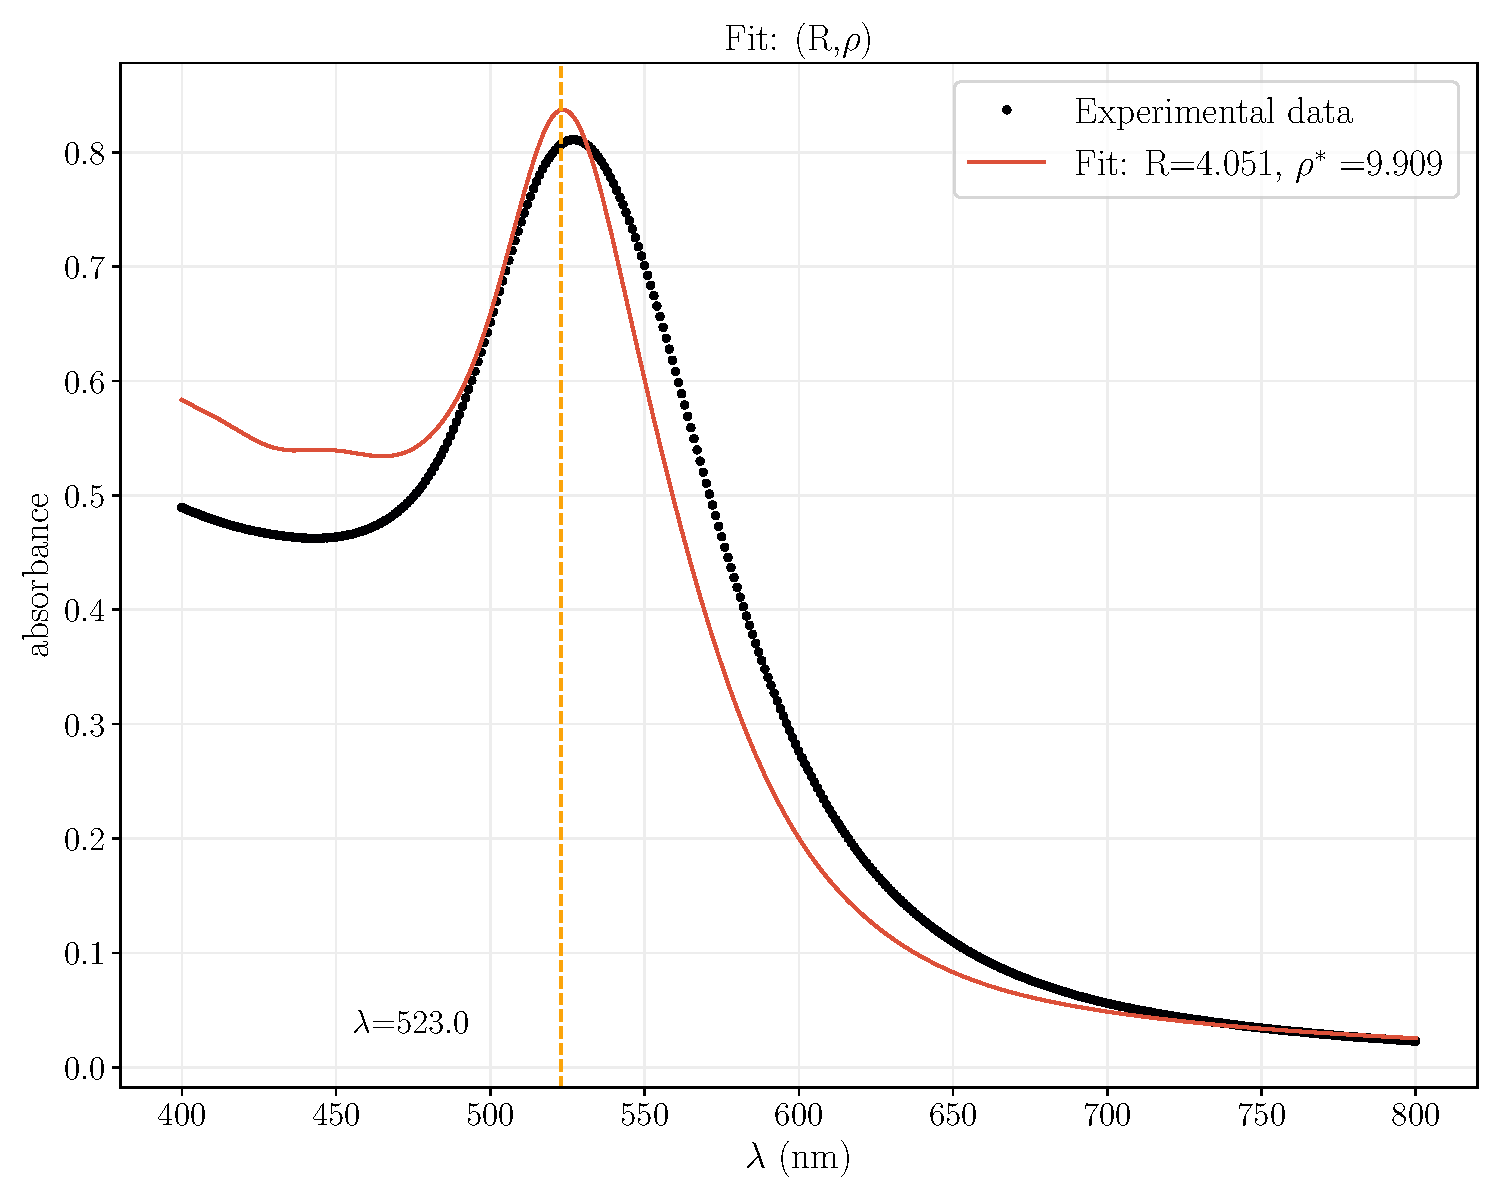
\includegraphics[width=.5\textwidth]{image/data/1_fit.pdf}} 
\subfloat[][{chi2}]
{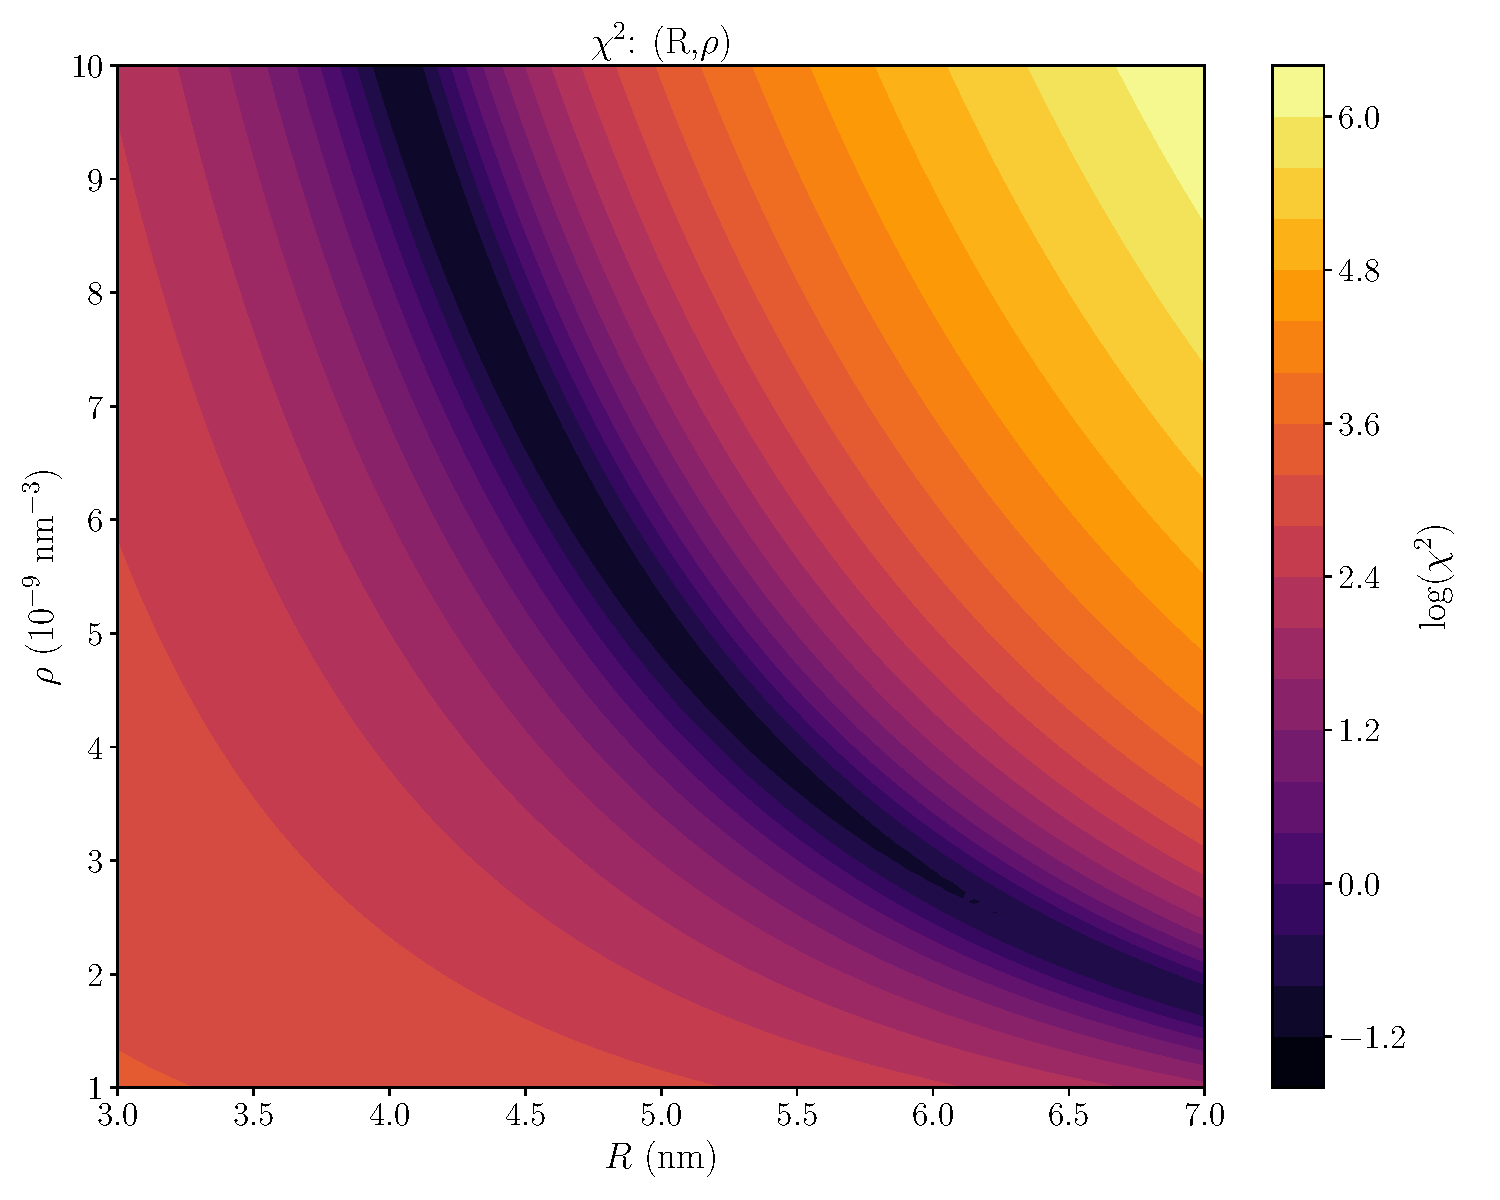
\includegraphics[width=.5\textwidth]{image/data/1_chisquare.pdf}} \\
\caption{questo è R,rho}
\label{fig:r_rho}
\end{figure}

\begin{figure}[H]
\centering
\subfloat[][{fit}]
{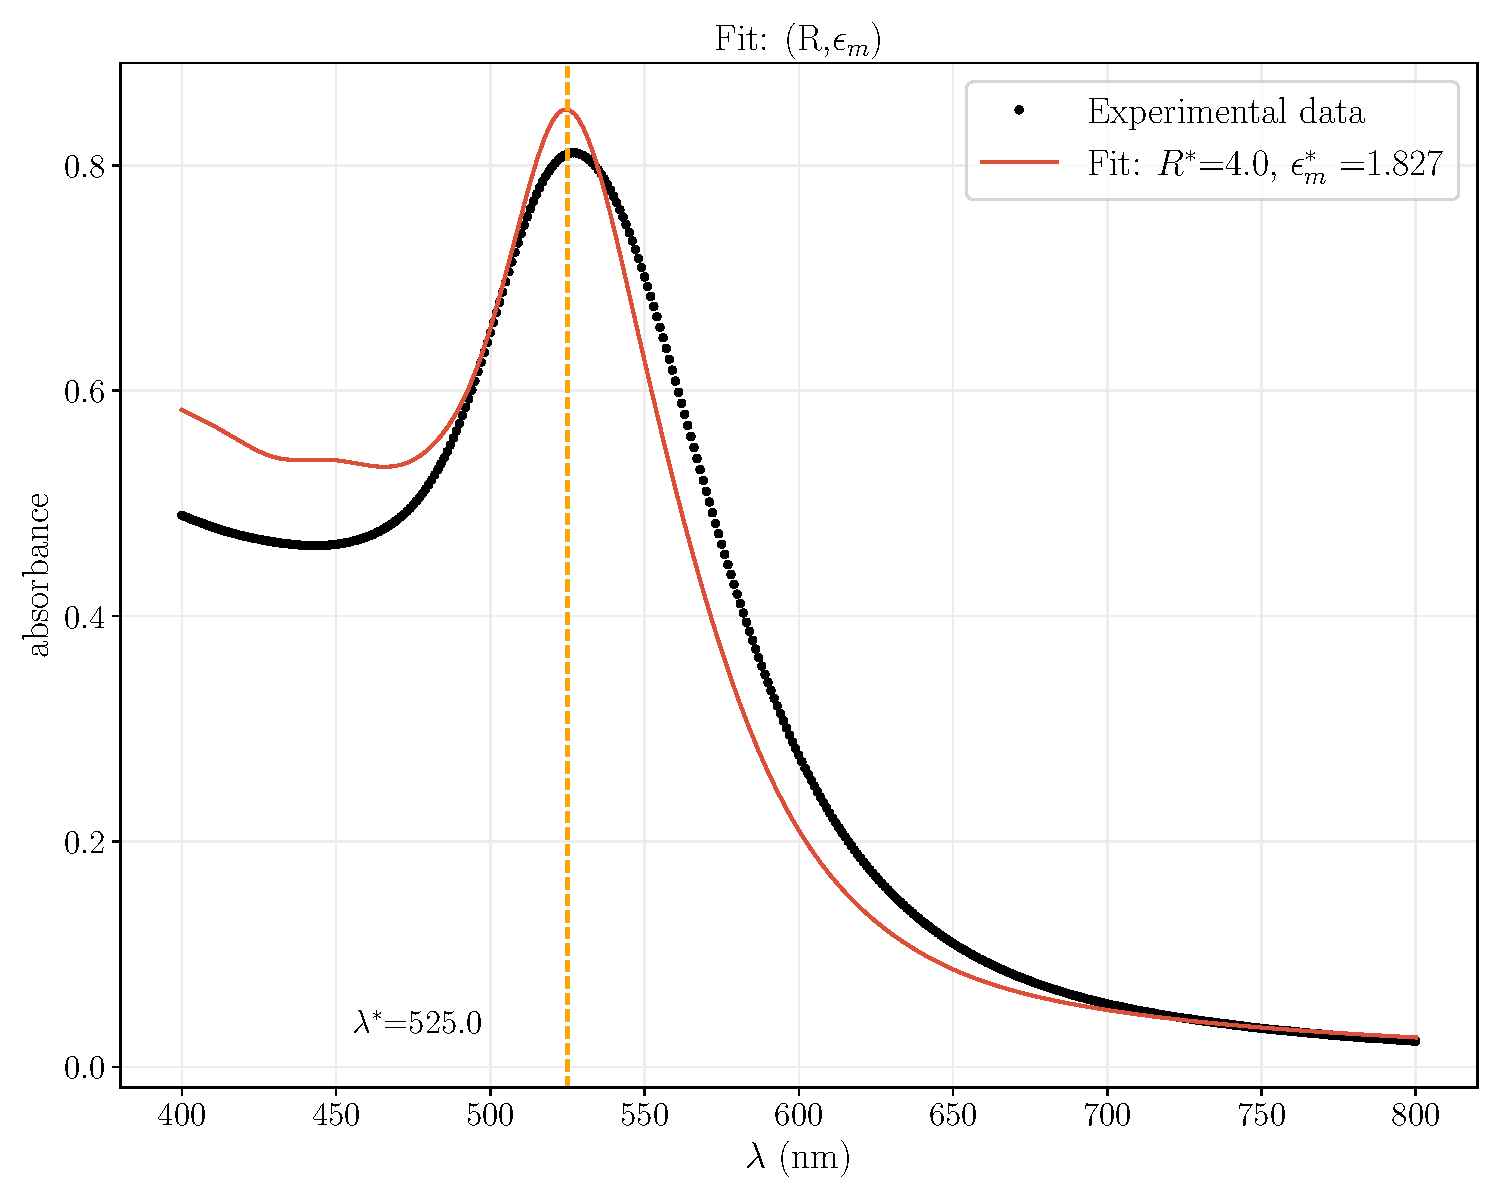
\includegraphics[width=.5\textwidth]{image/data/2_fit.pdf}} 
\subfloat[][{chi2 \gio{sistema il range del secondo fit! Può essere che però peggiori la stima di epsm}}]
{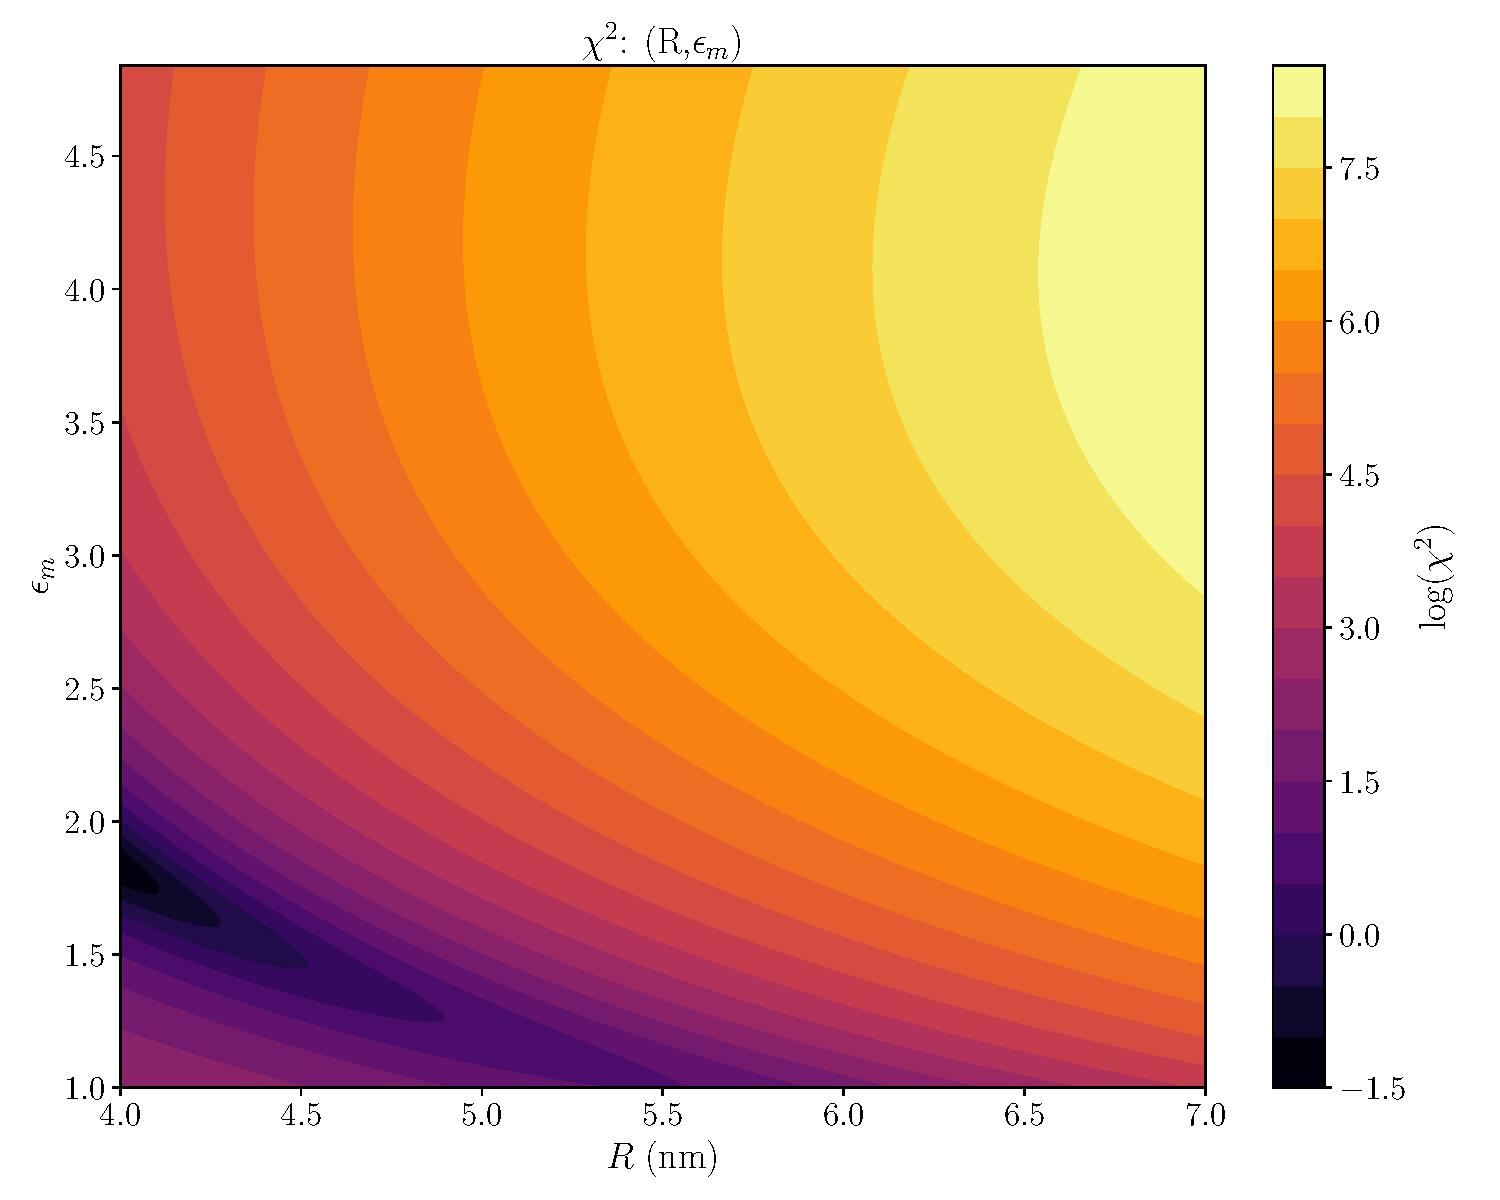
\includegraphics[width=.5\textwidth]{image/data/2_chisquare.pdf}} \\
\caption{questo è R,epsm}
\label{fig:r_epsm}
\end{figure}

\begin{multicols}{2}
\subsection{GANs Theory}

\begin{equation*}
\sigma_{ext}^{\text{Gans}} = \frac{\omega}{3c} \epsilon_m^{3/2}V_{0} \sum^{3}_{j=1}{\frac{\epsilon_2/L_j^2}{[\epsilon_1 + \epsilon_m(1-L_j)/L_j]^2 + \epsilon_2^2}}
\end{equation*}

The polarization coefficients $L_j$ are defined as 

\begin{subequations}
\begin{align}
  L_1 &= \frac{1-e^2}{e^2} \left[\frac{1}{2e}\ln{\left(\frac{1+e}{1-e}\right)}-1\right] \\
  L_2 &= L_3 = \frac{1-L_1}{2} 
\end{align}
\end{subequations}
where $e$ is the eccentricity.

\section{XRD Analysis}
\label{sec:XRD}

\subsection{Method}

\subsection{Results}

\section{SEM Analysis}
\label{sec:SEM}

\subsection{Method}

\subsection{Results}

\section{Conclusions}

\clearpage
\printbibliography

\end{multicols}

\end{document}